\documentclass[11pt]{article}

\usepackage[margin=1in]{geometry}
\usepackage{tikz}
\usetikzlibrary{arrows.meta, positioning, shapes.geometric, fit, backgrounds}
\usepackage{setspace}

\setstretch{1.05}

\begin{document}

\section*{System Architecture and Design}

This section presents the architecture of the proposed on-device intrusion detection and false alarm filtering system. The design emphasizes event-driven processing, real-time performance, and robustness under constrained hardware conditions, consistent with the requirement to operate on Windows-based systems with limited CPU and memory resources.

\begin{figure}[h!]
\centering
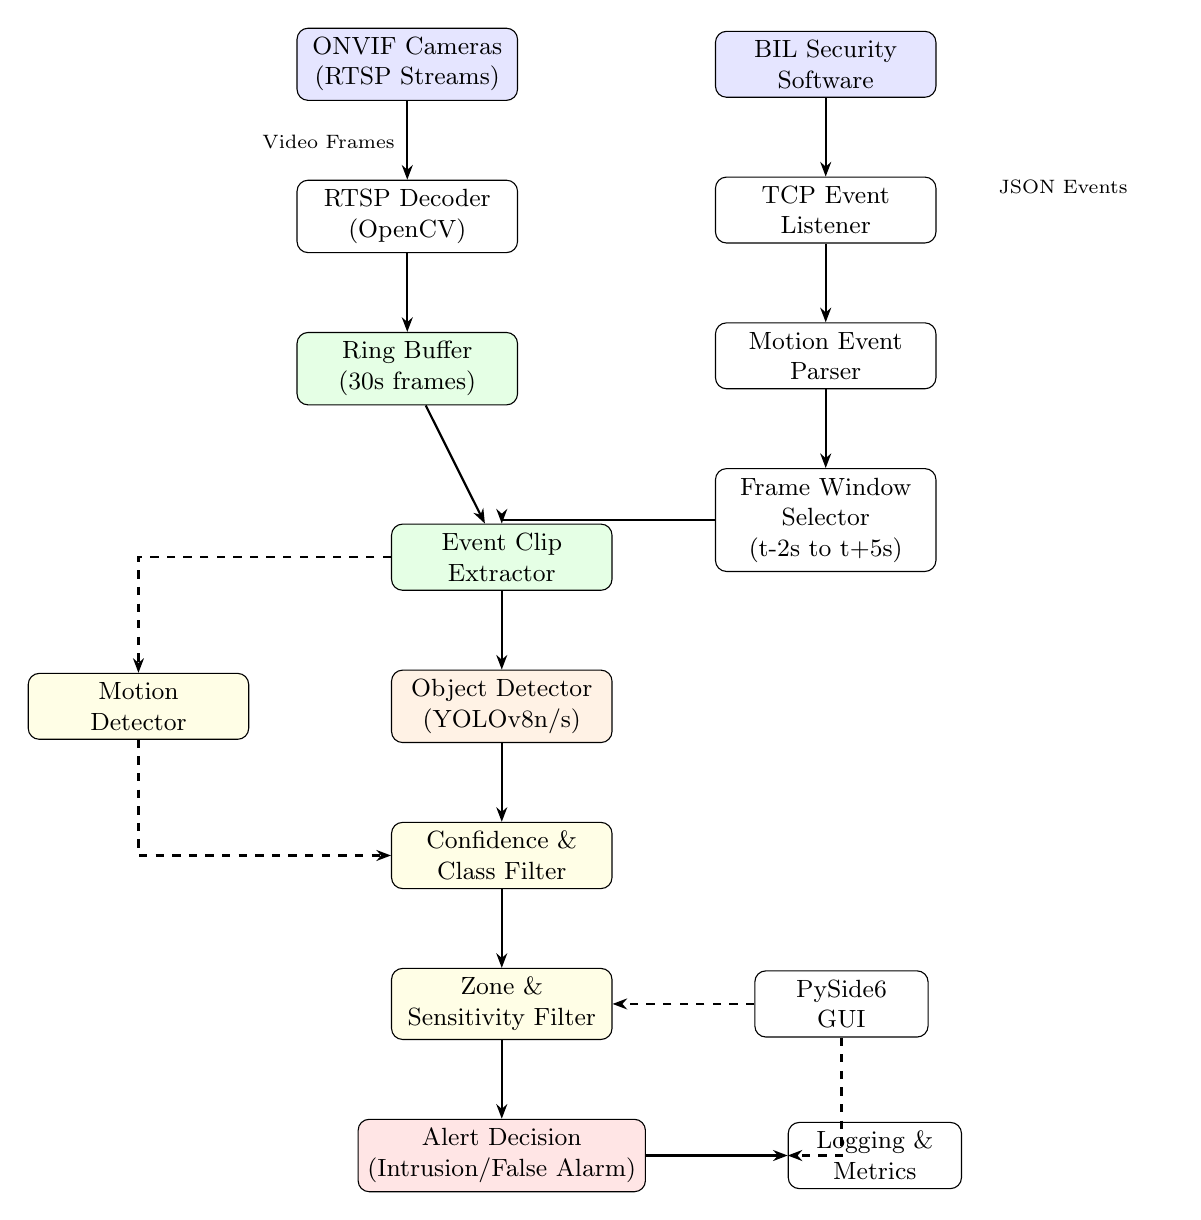
\begin{tikzpicture}[
    node distance=1.0cm and 2.2cm,
    every node/.style={
        draw,
        rectangle,
        rounded corners,
        align=center,
        minimum width=2.8cm,
        minimum height=0.75cm,
        font=\small
    },
    arrow/.style={-{Stealth[scale=0.8]}, thick},
    dashedarrow/.style={-{Stealth[scale=0.8]}, thick, dashed},
    external/.style={fill=blue!10},
    buffer/.style={fill=green!10},
    detect/.style={fill=orange!10},
    filter/.style={fill=yellow!10},
    output/.style={fill=red!10}
]

% === External Inputs (Top Row) ===
\node[external] (cameras) {ONVIF Cameras\\(RTSP Streams)};
\node[external, right=2.5cm of cameras] (bilsoftware) {BIL Security\\Software};

% === Ingest Layer ===
\node[below=of cameras] (rtsp) {RTSP Decoder\\(OpenCV)};
\node[below=of bilsoftware] (tcp) {TCP Event\\Listener};

% === Buffer Layer ===
\node[buffer, below=of rtsp] (ringbuffer) {Ring Buffer\\(30s frames)};

% === Event Processing ===
\node[below=of tcp] (eventparser) {Motion Event\\Parser};
\node[below=of eventparser] (windowselector) {Frame Window\\Selector\\(t-2s to t+5s)};

% === Clip Extraction ===
\node[buffer, below=1.5cm of ringbuffer, xshift=1.2cm] (clipextract) {Event Clip\\Extractor};

% === Detection Pipeline ===
\node[detect, below=of clipextract] (detector) {Object Detector\\(YOLOv8n/s)};
\node[filter, left=1.8cm of detector] (motiondet) {Motion\\Detector};

% === Filtering Layer ===
\node[filter, below=of detector] (postfilter) {Confidence \&\\Class Filter};
\node[filter, below=of postfilter] (zonefilter) {Zone \&\\Sensitivity Filter};

% === Output ===
\node[output, below=of zonefilter] (alertout) {Alert Decision\\(Intrusion/False Alarm)};

% === Logging/Metrics (side) ===
\node[right=1.8cm of alertout, minimum width=2.2cm] (logging) {Logging \&\\Metrics};

% === GUI (side) ===
\node[right=1.8cm of zonefilter, minimum width=2.2cm] (gui) {PySide6\\GUI};

% ============ ARROWS ============

% Camera path
\draw[arrow] (cameras) -- (rtsp);
\draw[arrow] (rtsp) -- (ringbuffer);
\draw[arrow] (ringbuffer) -- (clipextract);

% Event path
\draw[arrow] (bilsoftware) -- (tcp);
\draw[arrow] (tcp) -- (eventparser);
\draw[arrow] (eventparser) -- (windowselector);
\draw[arrow] (windowselector) -| (clipextract);

% Detection pipeline
\draw[arrow] (clipextract) -- (detector);
\draw[arrow] (detector) -- (postfilter);
\draw[arrow] (postfilter) -- (zonefilter);
\draw[arrow] (zonefilter) -- (alertout);

% Motion detector (optional path)
\draw[dashedarrow] (clipextract) -| (motiondet);
\draw[dashedarrow] (motiondet) |- (postfilter);

% Outputs
\draw[arrow] (alertout) -- (logging);
\draw[dashedarrow] (gui) -- (zonefilter);
\draw[dashedarrow] (gui) |- (logging);

% Labels for data flow
\node[draw=none, font=\scriptsize, above=0.1cm of rtsp, xshift=-1cm] {Video Frames};
\node[draw=none, font=\scriptsize, right=0.2cm of tcp, yshift=0.3cm] {JSON Events};

\end{tikzpicture}
\caption{Event-driven architecture for on-device intrusion detection. Solid arrows show the primary processing path; dashed arrows indicate optional/secondary paths.}
\end{figure}


\subsection*{Camera Input and Standards}
The system operates on security cameras compliant with ONVIF Profile S or Profile T standards. These profiles ensure standardized access to video streams via RTSP and reduce integration complexity by providing predictable streaming behavior across supported devices. Video streams are decoded using OpenCV's VideoCapture and stored in a ring buffer.

\subsection*{TCP Motion Event Handling}
Motion events are received from existing BIL Security software via an asynchronous TCP listener (port 9000). Each event contains a camera identifier and timestamp in JSON format, allowing the system to align incoming events with buffered video frames. This enables event-driven inference, where expensive processing is performed only when motion is reported by the external system.

\subsection*{Ring Buffer and Frame Storage}
A thread-safe ring buffer maintains a 30-second sliding window of timestamped frames for each camera. This design allows the system to retrospectively access frames from before an event occurred, which is essential for capturing the full context of an intrusion.

\subsection*{Frame Window Selection}
Upon receiving a motion event at time $t_e$, the Event Frame Window Selector extracts a bounded window of frames spanning $t_e - 2$ seconds to $t_e + 5$ seconds. This 7-second window provides sufficient temporal context while limiting computational overhead. At 15 FPS with frame skipping (every 3rd frame), approximately 35 frames are analyzed per event.

\subsection*{Object Detection}
Extracted frames are processed by a lightweight object detector. Based on benchmarking at native HD resolution (1280$\times$720), YOLOv8 Nano is the recommended model:

\begin{center}
\begin{tabular}{|l|c|c|c|}
\hline
\textbf{Model} & \textbf{FPS @ 720p} & \textbf{Detections/Frame} & \textbf{Recommendation} \\
\hline
YOLOv8n & 20.4 & 7 & Primary choice \\
YOLOv8s & 13.7 & 9 & Maximum accuracy \\
MobileNet-SSD & 15.5 & 5 & Legacy only \\
\hline
\end{tabular}
\end{center}

A key finding is that MobileNet-SSD, while faster at lower resolutions, performs 31\% slower than YOLOv8n at native HD resolution due to internal resizing overhead.

\subsection*{Motion Detection (False Alarm Filter)}
An optional motion detection stage using background subtraction (MOG2) and frame differencing provides secondary validation. By requiring both object detection AND motion detection, the system filters:
\begin{itemize}
    \item Stationary objects (parked cars, furniture) that appear in detection but not motion
    \item Environmental motion (weather, vegetation) that appears in motion but not as person/vehicle detections
\end{itemize}

\subsection*{Confidence and Class Filtering}
Raw detections are filtered by confidence threshold and restricted to alert classes (person, car, truck, bus, motorcycle, bicycle). Temporal consistency may be enforced by requiring detections to persist across multiple frames.

\subsection*{Zone and Sensitivity Filtering}
User-defined polygon zones restrict monitoring to specific regions of interest. Detections outside enabled zones are filtered out. The GUI provides an interactive zone editor where users can draw monitoring regions by clicking points to form polygons.

\subsection*{Alert Output and Logging}
Final decisions classify each event as either a valid intrusion or a filtered false alarm. Results are logged with performance metrics including processing latency, detection counts, and false alarm rates.

\subsection*{Event-Driven Processing Advantage}
The event-driven architecture fundamentally changes hardware requirements compared to real-time streaming:

\begin{center}
\begin{tabular}{|l|l|c|}
\hline
\textbf{Architecture} & \textbf{FPS Requirement} & \textbf{CPU-Only Viable?} \\
\hline
Real-Time (10 cameras $\times$ 15fps) & 150 FPS continuous & No \\
Event-Driven Clips & $\sim$35 frames per event & Yes \\
\hline
\end{tabular}
\end{center}

With event-driven processing, a single event takes approximately 1.7 seconds to analyze with YOLOv8n, providing capacity for $\sim$35 events per minute---more than sufficient for typical surveillance scenarios where motion events are sporadic.

\subsection*{GUI and User Interface}
A PySide6-based graphical interface provides:
\begin{itemize}
    \item Camera configuration and status monitoring
    \item Interactive zone editor with polygon drawing
    \item Test panel for video/webcam detection testing
    \item Alert log with filtering by object type, zone, and confidence
    \item Model selection and sensitivity settings
\end{itemize}

\end{document}
